\subsection{Motivation}
\label{chp:stylometry_extensions:followingTrail:motivation}
In~\chapref{chp:sysml}, we described an architecture utilizing text CNNs~\citep{kim2014convolutional} for generating the textual component of representations for authorship attribution on darknet forums.
Recent work on generalizing authorship representations has focused on a variation of the popular sentence transformer architecture~\citep{reimers2019sentencebert}.
Specifically, \citet{riverastao2021learning} compared the transferability of author representation learning models between Amazon reviews, fanfiction short stores, and Reddit comments.
They found that in a zero-shot setting, i.e., without any addition in domain data, the models trained on Reddit data had the highest degree of generalization to new domains.
This work motivates us to explore the generalization capabilities of models trained on clear web data to dark web forums.
We explore two research questions.
First, can we apply author representation models trained on Reddit forum data directly to Darkweb forums?
Second, can we combine data from the dark web and clear web to build better models?

\subsection{Methodology}
\label{chp:stylometry_extensions:followingTrail:methodology}

\begin{figure*}
    \centering
    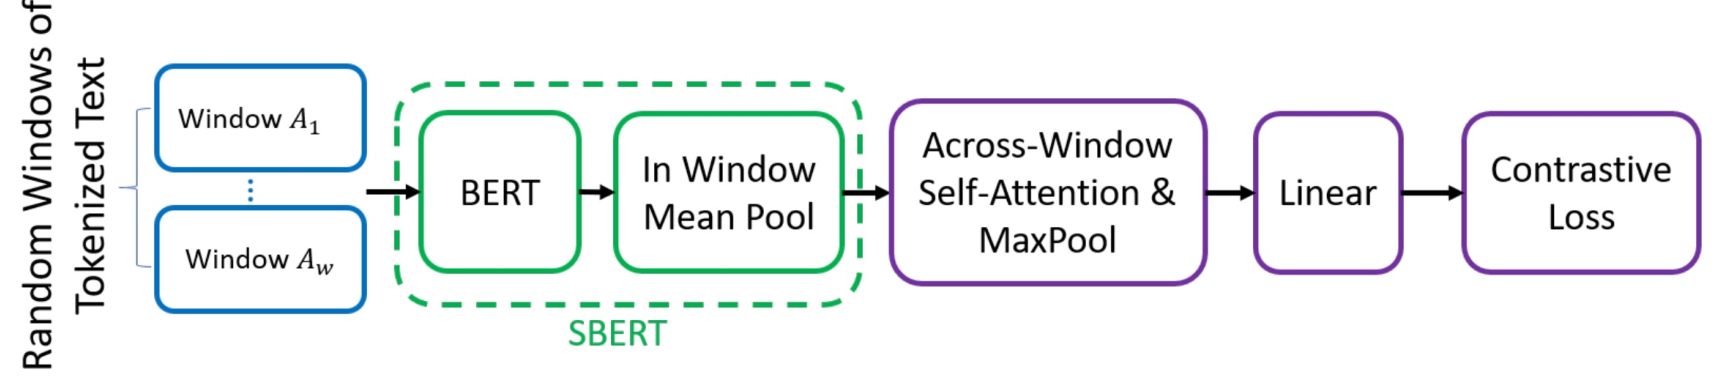
\includegraphics[width=\linewidth]{stylometryExtensions/figures/LUAR.pdf}
    \caption{Architecture for LUAR~\citep{riverastao2021learning}}
    \label{fig:stylometry_extensions:followingTrail:LUAR}
\end{figure*}